% -----------------------------------------------
% Template for ICMC SMC 2014
% adapted and corrected from the template for SMC 2013,  which was adapted from that of  SMC 2012, which was adapted from that of SMC 2011
% -----------------------------------------------

\documentclass{article}
\usepackage{icmcsmc2014}
\usepackage{times}
\usepackage{ifpdf}
\usepackage[english]{babel}
%\usepackage{cite}

%%%%%%%%%%%%%%%%%%%%%%%% Some useful packages %%%%%%%%%%%%%%%%%%%%%%%%%%%%%%%
%%%%%%%%%%%%%%%%%%%%%%%% See related documentation %%%%%%%%%%%%%%%%%%%%%%%%%%
%\usepackage{amsmath} % popular packages from Am. Math. Soc. Please use the
%\usepackage{amssymb} % related math environments (split, subequation, cases,
%\usepackage{amsfonts}% multline, etc.)
%\usepackage{bm}      % Bold Math package, defines the command \bf{}
%\usepackage{paralist}% extended list environments
%%subfig.sty is the modern replacement for subfigure.sty. However, subfig.sty
%%requires and automatically loads caption.sty which overrides class handling
%%of captions. To prevent this problem, preload caption.sty with caption=false
%\usepackage[caption=false]{caption}
%\usepackage[font=footnotesize]{subfig}


%user defined variables
\def\papertitle{Flocking: A Framework for Declarative Music-Making on the Web}
\def\firstauthor{Colin Clark}
\def\secondauthor{Adam Tindale}
\def\thirdauthor{nobody}
% adds the automatic
% Saves a lot of ouptut space in PDF... after conversion with the distiller
% Delete if you cannot get PS fonts working on your system.

% pdf-tex settings: detect automatically if run by latex or pdflatex
\newif\ifpdf
\ifx\pdfoutput\relax
\else
   \ifcase\pdfoutput
      \pdffalse
   \else
      \pdftrue
\fi

\ifpdf % compiling with pdflatex
  \usepackage[pdftex,
    pdftitle={\papertitle},
    pdfauthor={\firstauthor, \secondauthor},
    bookmarksnumbered, % use section numbers with bookmarks
    pdfstartview=XYZ % start with zoom=100% instead of full screen;
                     % especially useful if working with a big screen :-)
   ]{hyperref}
  %\pdfcompresslevel=9

  \usepackage[pdftex]{graphicx}
  % declare the path(s) where your graphic files are and their extensions so
  %you won't have to specify these with every instance of \includegraphics
  \graphicspath{{./figures/}}
  \DeclareGraphicsExtensions{.pdf,.jpeg,.png}

  \usepackage[figure,table]{hypcap}

\else % compiling with latex
  \usepackage[dvips,
    bookmarksnumbered, % use section numbers with bookmarks
    pdfstartview=XYZ % start with zoom=100% instead of full screen
  ]{hyperref}  % hyperrefs are active in the pdf file after conversion

  \usepackage[dvips]{epsfig,graphicx}
  % declare the path(s) where your graphic files are and their extensions so
  %you won't have to specify these with every instance of \includegraphics
  \graphicspath{{./figures/}}
  \DeclareGraphicsExtensions{.eps}

  \usepackage[figure,table]{hypcap}
\fi

%setup the hyperref package - make the links black without a surrounding frame
\hypersetup{
    colorlinks,%
    citecolor=black,%
    filecolor=black,%
    linkcolor=black,%
    urlcolor=black
}


% Title.
% ------
\title{\papertitle}

% Authors
% Please note that submissions are NOT anonymous, therefore
% authors' names have to be VISIBLE in your manuscript.
%
% Single address
% To use with only one author or several with the same address
% ---------------
%\oneauthor
%   {\firstauthor} {Affiliation1 \\ %
%     {\tt \href{mailto:author1@smcnetwork.org}{author1@smcnetwork.org}}}

%Two addresses
%--------------
 \twoauthors
   {\firstauthor} {OCAD University \\ %
     {\tt \href{mailto:cclark@ocadu.ca}{cclark@ocadu.ca}}}
   {\secondauthor} {OCAD University \\ %
     {\tt \href{mailto:atindale@faculty.ocadu.ca}{atindale@faculty.ocadu.ca}}}

% Three addresses
% --------------
% \threeauthors
%   {\firstauthor} {Affiliation1 \\ %
%     {\tt \href{mailto:author1@smcnetwork.org}{author1@smcnetwork.org}}}
%   {\secondauthor} {Affiliation2 \\ %
%     {\tt \href{mailto:author2@smcnetwork.org}{author2@smcnetwork.org}}}
%   {\thirdauthor} { Affiliation3 \\ %
%     {\tt \href{mailto:author3@smcnetwork.org}{author3@smcnetwork.org}}}


% ***************************************** the document starts here ***************
\begin{document}
%
\capstartfalse
\maketitle
\capstarttrue
%
\begin{abstract}
Flocking\footnote{http://flockingjs.org/} is a framework for audio synthesis and music composition written in JavaScript. It takes a unique approach to solving several of the common architectural problems faced by computer music environments, emphasizing a declarative style that is closely aligned with the principles of the web.

In Flocking, instruments and scores are defined as JavaScript Object Notation (JSON) objects. JSON is a subset of the JavaScript language that is used widely across the web for exchanging data. By representing the basic building blocks of synthesis declaratively, Flocking’s goal is to enable the growth of an ecosystem of tools that can easily parse and understand the logic and semantics of digital instruments. This is particularly useful for supporting generative composition (where programs generate new instruments and scores algorithmically), graphical tools (for programmers and non-programmers alike to collaborate), and new modes of social programming that allow musicians to easily adapt, extend, and rework existing instruments without having to ``fork" their code.

In contrast to other emerging web audio libraries and tools, Flocking provides a robust, optimized, and well-tested architecture that explicitly supports extensibility and long-term growth. Flocking runs in nearly any modern JavaScript environment, including desktop and mobile browsers (Chrome, Firefox, and Safari), as well as on embedded devices with Node.js.

\end{abstract}
%

\section{Introduction}\label{sec:introduction}

Many computer music programming tools have been developed to enable musicians, composers, artists, students, and explorers to engage with music through code. Each tool attempts solves a particular problem of efficiency, expressivity, or portability. Many aim to make advances in all three areas - Flocking is a new computer music programming framework that aims to achieve exactly this.

This paper will demonstrate Flocking's expressivity with a discussion of the declarative paradigm utilized, efficiency with a discussion of optimization tactics for JavaScript web audio toolkits and a comparison with other libraries, and portability with a discussion of the underlying framework and Flocking's ability to communicate with other tools (GUI, MIDI, OSC, etc).

Flocking is a programming framework rather than a programming language or environment. It is implemented in JavaScript to make it available to a broad range of platforms and to fit naturally into the wider ecosystem of web tools.

\section{The Approach}

\subsection{Why Use The Web?}

Much computer music research over the past few decades has focused on {\it syntax} and the idea that what computer musicians need most are new syntactic ways to express musical and time-based constructs programmatically \cite{dannenberg2002language}. Though this emphasis on syntax has produced noteworthy computer music languages (e.g. SuperCollider, ChucK, Aura, etc.) and useful results for use cases such as live coding, the preponderance of isolated, specialist programming languages for music and art has led to, in the opinion of the first author, a disconnect between creative coders and the mainstream world of software developers. SuperCollider, as an example of a very successful musician-specialist programming language, provides myriad ways to express time-based concepts, yet it continues to be difficult to create polished user interfaces or to connect with web-based services and sources of data---tasks that are trivial in mainstream programming environments such as JavaScript. As the world of interconnected devices, sensors, and participatory software increases, these limitations take an increasing toll on the complexity of creative coding, serving to separate musicians and artists from other programmers working in the field.

In order to address this concern, Flocking was conceived from the beginning as a means for connecting musicians and artists up with the cross-platform, distributed delivery model of the web, along with the larger pool of libraries, user interface components, and tutorials that are available to the web development community.

\subsection{A Declarative Ecosystem}

Another motivating concern for Flocking is that the prevailing emphasis on syntax has shifted focus away from interoperability amongst tools and systems within an open computer music ecosystem. Today, binary oppositions prevail; a prospective computer musician typically must choose from the outset whether or not she wants to use a code-based environment (such as CSound, SuperCollider, or ChucK) or a graphical one (Max/MSP or PD, for example). Since imperative programming code can't easily be parsed or generated by tools outside the chosen environment, the code and graphical paradigms rarely interoperate. As a result, it is difficult for musicians to collaborate on a project across modalities. Tools such as Open Sound Control \cite{wright1997open} significantly help with cross-system interoperability at runtime, and some environments such as Max support the embedding of programmatic code ``externals" within an otherwise graphical instrument. Nonetheless, these solutions don't allow programmers and non-programmers alike to collaborate on the same underlying instruments and scores.

Flocking's use of declarative programming idioms, which are discussed in more detail below, is intended to support {\it metaprogramming}, enabling new kinds of both graphical and textual tools within the larger context of web-based music. Alternative bindings to Flocking's declarative formats could also be created, allowing instruments to be shared across computer music languages. There is significant work still to be done in this regard---a prototype code and graphical development environment for Flocking is still in early development---but the declarative approach provides a foundation for deeply exploring the issue of interoperability and collaboration.

\subsection{Common Abstractions}

Another challenge that computer music systems face is how to model the architectural distinction between different types of changes that occur at varying time scales. Such changes include:

\begin{enumerate}
\item highly optimized data flow-based changes that occur at the signal level
\item value or instrument changes scheduled at fixed or indeterminate rates (a ``score")
\item messages or events sent between objects in an object-oriented system
\item user-triggered events from an OSC or MIDI controller, or from graphical user interface components such as buttons and knobs
\end{enumerate}

Different computer music systems take radically different approaches to modelling these distinctions. For example, Max historically supported only an event-based approach that was optimized for changes coming from an external controller; signal processing was added later as a special type of message \cite{puckette2002max}.
SuperCollider, on the other hand, makes a semantic and syntactic distinction between the signal-level changes performed by unit generators on the server \cite{mccartney1996supercollider} and {\it Patterns}, which form a completely different abstraction for change \cite[pp. 189]{wilson2011supercollider}.

Born out of frustration with these overlapping, incompatible abstractions in SuperCollider---both of which attempt to represent sources of changing values over time---Flocking aims to smooth over this systemic distinction between signal-level events and scheduled events. It does this by adopting a single, unified representation of change. In Flocking, value changes within an instrument and changes that are scheduled as part of the compositional structure of a piece are both represented as trees of unit generators. The only difference is the rate at which these unit generators are evaluated. A single abstraction for change provides less ``conceptual surface" for newcomers to learn, and enables instruments to be used in different contexts, both at the macro and micro levels. This topic is discussed further, with examples, in the \ref{sec:Scheduling} section.

\section{How Flocking Works}

\subsection{The Framework}

The core of the Flocking framework consists of several interconnected components that provide the essential behaviour of interpreting and instantiating unit generators, producing streams of samples, and scheduling changes. Flocking's primary components include:

\begin{enumerate}
\item the {\it Flocking interpreter}, which parses and instantiates synths, unit generators, and buffers
\item the {\it Environment}, which represents the overall audio system and its configuration settings
\item {\it Audio Strategies}, which are pluggable audio output adaptors (binding to backends such as the Web Audio API or ALSA on Node.js)
\item {\it Unit Generators} (ugens), which are the sample-generating primitives used to produce sound
\item {\it Synths}, which represent instruments and collections of signal-generating logic
\item the {\it Scheduler}, which manages time-based change events on a synth
\end{enumerate}

The following diagram shows the runtime relationships between the components that comprise the Flocking framework, showing an example of how multiple synths and unit generators are composed into a single Web Audio ScriptProcessorNode.

\begin{figure}[h]
\centering
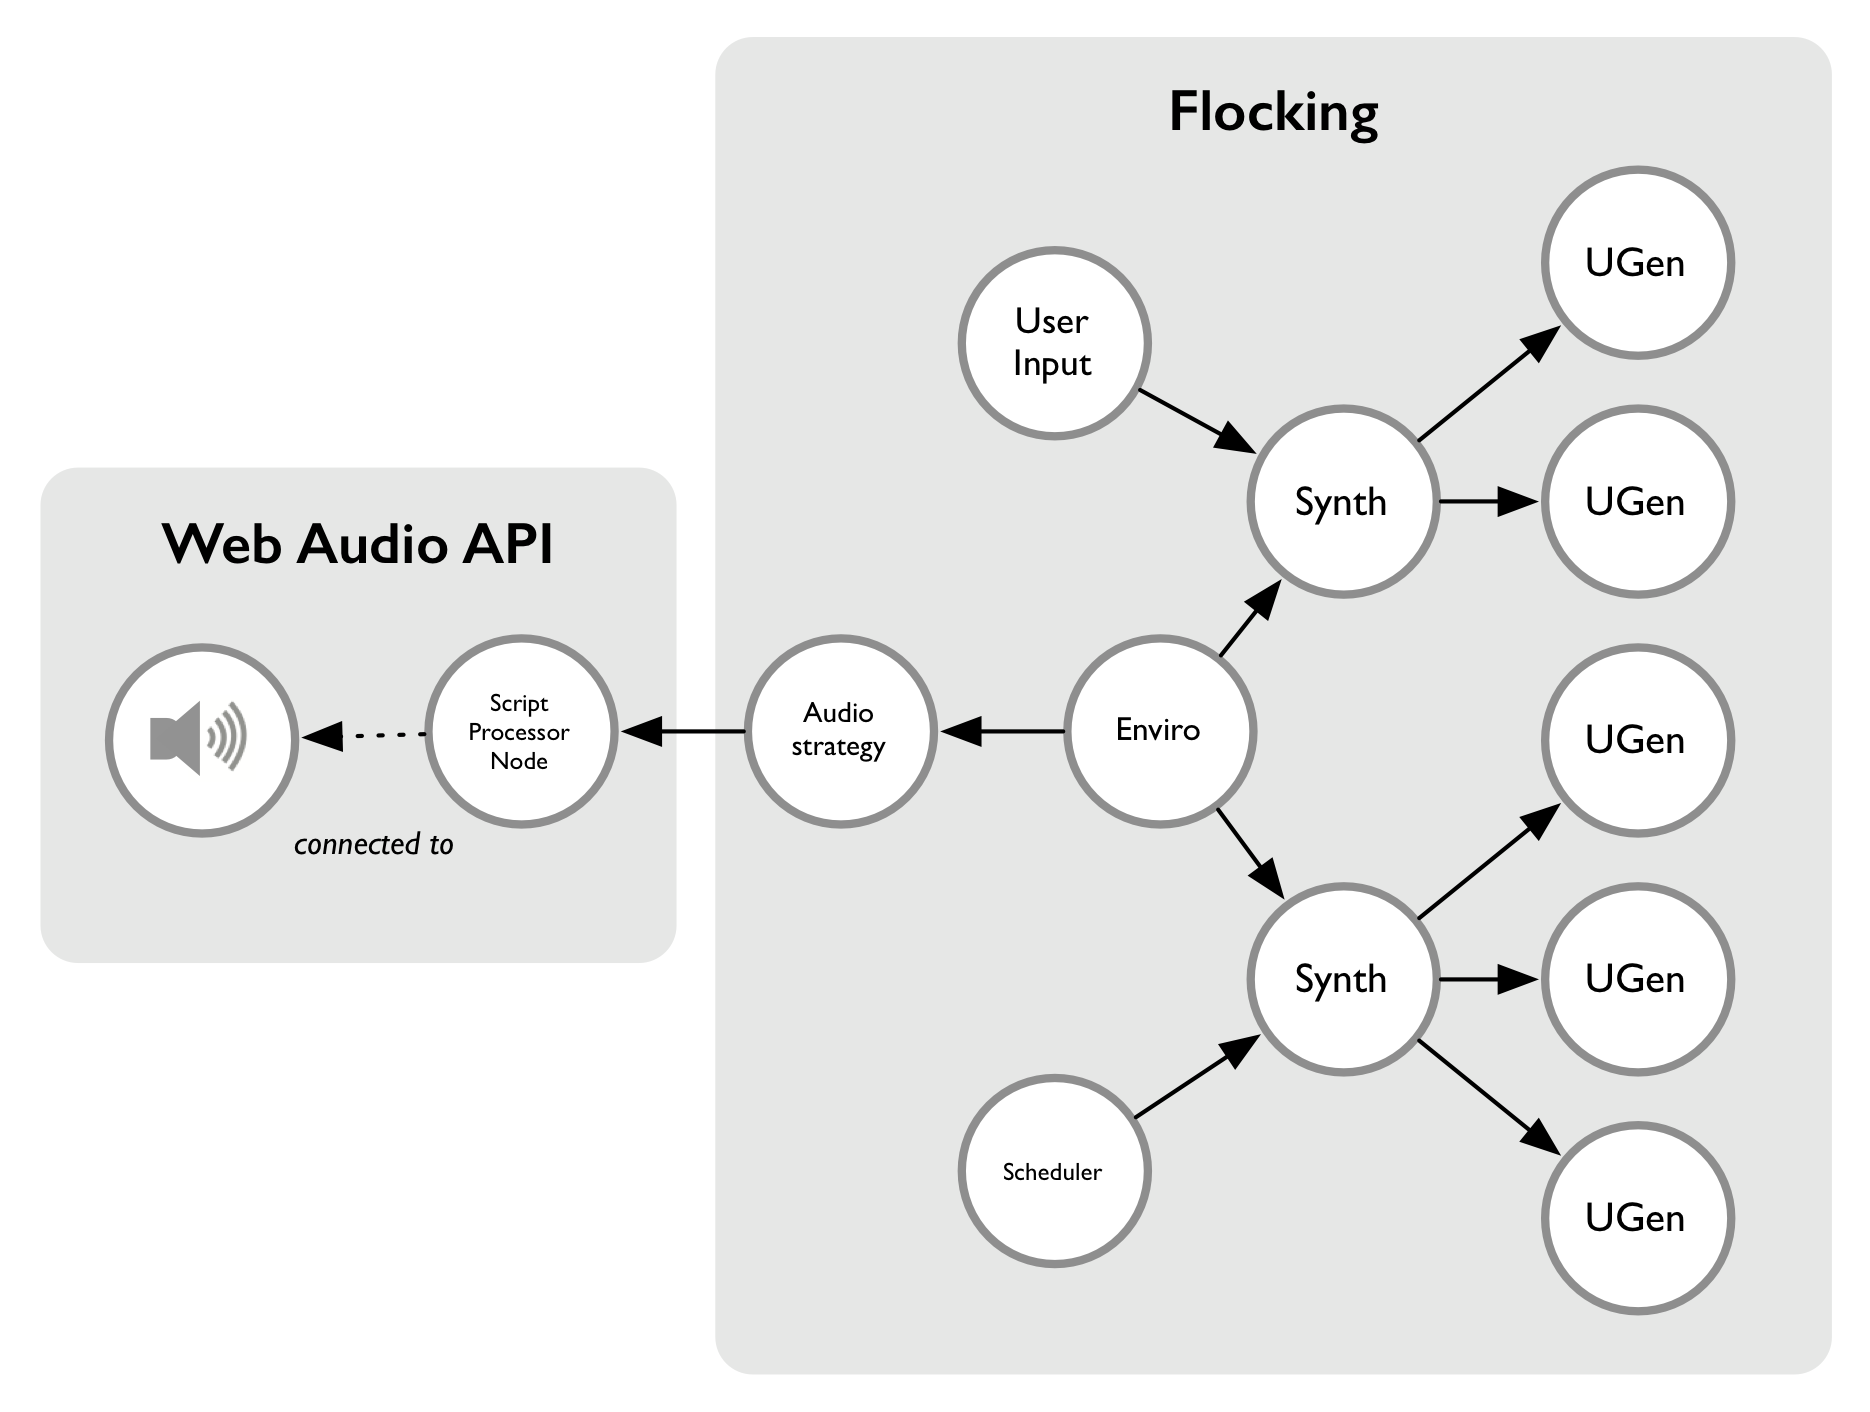
\includegraphics[width=0.9\columnwidth]{images/flocking-component-architecture.png}
\caption{ A diagram showing Flocking's primary components and how they relate to each other and to the Web Audio API.\label{fig:architecture}}
\end{figure}

\subsection{Declarative Programming}

We described Flocking above as a declarative framework, and this characteristic is essential to understanding its design. Declarative programming can be understood in the context of Flocking as having two essential aspects:

\begin{enumerate}
\item it emphasizes a high-level, semantic view of a program’s logic and structure
\item it represents programs as data structures that can be understood by other programs
\end{enumerate}

J.W. Lloyd's informal definition of declarative programming is probably the most helpful starting point for establishing a pragmatic understanding of the first point. ``Declarative programming involves stating {\it what} is to be computed but not necessarily {\it how} it is to be computed" \cite{lloyd1994practical}. The emphasis here is on the logical or semantic aspects of computation, rather than on low-level sequencing and control flow. For musicians, the familiar unit generator abstraction established in the 1950s by Max Mathews in Music IV \cite{mathews1969technology} offers a partial example of the declarative approach. Unit generators represent a higher-level abstraction for audio signals; they are building blocks that a musician specifies and connects together. In this model, the musician doesn't directly specify the line-by-line sequencing of how a sine wave, for example, is produced. Rather, she declares the desired signal-generating processes by name and lets the synthesis environment do the rest.

The second point, relating to the use of common data structures to represent programs, is the more subtle and also more significant aspect of Flocking’s declarative design. Traditional imperative programming styles are typically intended for an ``audience of one"---the compiler. Though code is often shared amongst multiple developers, it can’t typically be understood or manipulated by programs other than the compiler.

In contrast, declarative programming involves the ability to write programs that are represented in a format that can be processed by other programs as ordinary data. The Lisp family of languages are a well-known example of this approach. Paul Graham describes the declarative nature of Lisp, saying it ``has no syntax. You write programs in the parse trees... [that] are fully accessible to your programs. You can write programs that manipulate them... programs that write programs." Though Flocking is written in ordinary JavaScript, it shares with Lisp the approach of expressing programs within data structures (written as JSON) that are fully available for manipulation by other programs.

\subsection{JSON}

The key to Flocking's declarative approach is JSON, the JavaScript Object Notation format. JSON is a lightweight data interchange format based on a subset of JavaScript that can be parsed and manipulated in nearly any programming language (Crockford {\it json.org}). JSON provides several primary data type and structures that are practically universal across programming languages. The following table describes these data structures and their syntax:

\begin{tabular}{| c || c | c |}
    \hline
    \bf{Type} & \bf{Syntax} & \bf{Description} \\ \hline
    Object & \verb|{}| & Associative array of key/value pairs \\ \hline
    Array & \verb|[]| & An ordered list \\ \hline
    String & \verb|"cat"| & A character sequence \\ \hline
    Number & \verb|440.4| & A floating point number \\ \hline
\end{tabular}

Since JSON's syntax and semantics are identical to JavaScript's own type literals, JSON is an exceptionally convenient language for representing data in web applications without requiring additional parsing complexity. All of Flocking's musical primitives are expressed as trees of JSON objects. These objects can be trivially serialized, traversed, manipulated, and merged with other objects.

In comparison to other music programming environments, which often describe themselves as functional or object-oriented, Flocking weaves the two approaches together in a manner that could be called ``document-oriented." Where Max and PD provide compositionality by creating patch objects, and SuperCollider and ChucK provide this with functions, Flocking enables exceptional compositionality through the creation of ``documents" (declarative JSON specifications) that can be reused and extended with a simple document merging algorithm provided by the framework.

\subsection{Unit Generator Definitions}

Musicians working with Flocking don't typically instantiate unit generators directly. Instead, they compose JSON objects into trees. Each node in the tree, called {\it unit generator definitions} (ugenDefs), describes a unit generator and its connection to others in the signal-processing graph. A ugenDef includes the following information:

\begin{enumerate}
\item the type of unit generator that should be instantiated
\item a named set of inputs (as key/value pairs), which can consist of either literal values (floats) or other unit generator specifications
\item a named set of static options, which describe how the unit generator should be configured
\end{enumerate}

Below is a simple example of a sine wave oscillator, illustrating how a Flocking unit generator is defined in JSON:

\begin{verbatim}
{
  ugen: "flock.ugen.sinOsc",
  inputs: {
    freq: 440,
    mul: 0.25
  },
  options: {
    interpolation: "linear"
  }
}
\end{verbatim}

Unit generator types are expressed as dot-separated strings called {\it key paths} or {\it EL expressions}. These strings are bound to creator functions at instantiation time by Flocking. All type expressions refer to a global namespace hierarchy so that developers can easily contribute their own unit generator implementations (using their own namespace to avoid conflicts) and have the Flocking framework manage them in the same manner as any of the built-in types.

\subsection{Synth Definitions}

A collection of unit generator definitions form the basis for a {\it synth definition} (synthDef). Synth definitions describe a complete instrument to be instantiated by the Flocking framework. Synths typically include a connection to an output bus---either the speakers or a shared ``interconnect" bus. In this respect, Flocking's architecture is highly inspired by SuperCollider (cite SuperCollider book page 25). Here is a simple example of a synthDef that outputs two sine waves, one in each stereo channel:

\begin{verbatim}
{
  ugen: "flock.ugen.out",
  sources: [
    {
      ugen: "flock.ugen.sinOsc"
    },
    {
      ugen: "flock.ugen.sinOsc",
      freq: 444
    }
  ]
}
\end{verbatim}

This example illustrates a key aspect of Flocking's interpreter and its document-merging approach. In the case of the first unit generator, we have omitted all input values. When the synth is actually played, it will automatically be given a frequency of 440 Hz. This is due to the fact that every built-in unit generator declares a set of default values. The Flocking interpreter, prior to instantiating the unit generator, will merge the user's ugenDef values on top of the defaults. If a property is omitted, the default value will be retained; if a user specified a property, it will be omitted. To save typing, the interpreter will also handle input names correctly when they aren't nested inside an ``inputs" container.

To actually instantiate a Synth, its creator function must be called. In Flocking, a component creator function typically takes only one argument---the component's {\it options} structure---and returns an instance of the component. In the case of Synths, the options object must include the synthDef as well as any other settings needed to appropriately configure the synth instance. Here is an example of how to create a Flocking synth programmatically:

\begin{figure}[h!]
    \begin{verbatim}
var synth = flock.synth({
  synthDef: {
    id: "carrier",
    ugen: "flock.ugen.sinOsc",
    freq: 440,
    phase: {
      id: "mod",
      ugen: "flock.ugen.sinOsc",
      freq: 34.0,
      mul: {
        ugen: "flock.ugen.sinOsc",
        freq: 1/20,
        mul: flock.PI
      },
      add: flock.PI
    },
    mul: 0.25
  }
});
    \end{verbatim}
    \caption{Instantiating a custom phase modulation synth.\label{fig:pmSynth}}
\end{figure}


By default, synths are automatically added to the tail of the Environment's list of nodes to evaluate, so they will start sounding immediately if the Environment has been started. Synths also respond to \verb|play| and \verb|pause| messages; a call to \verb|play()| will add the synth and start the environment if necessary.

\subsection{Updating Values}

Once a synth has been instantiated, its inputs can be changed on the fly. Flocking supports a highly dynamic signal processing pipeline; unit generators can be added or swapped out from a synth at any time, even while it's playing. Behind the scenes, everything in the signal graph is actually a unit generator, even static values.

In order to direct changes at a particular unit generator, it has to be given an identifying name. In the example shown in figure \ref{fig:pmSynth}, the carrier and modulator unit generators are each given an ``id" property which names them. These represent ``cutpoints" into the overall tree to enable easier access to a particular unit generator. Synths keep track of all their named unit generators and provide \verb|get()| and \verb|set()| methods for making programmatic changes to a synth's values.

Changes can be targeted at any unit generator within the tree by using key path expressions. Here's an example of how multiple changes can be made to different points in the unit generator tree with a single call to \verb|Synth.set()|:

\begin{verbatim}
  synth.set({
    "carrier.freq": 220,
    "mod.mul.freq": 1/30
  });
\end{verbatim}

This example lowers the frequency of the carrier oscillator by an octave while simultaneously slowing down the rate that the modulator's amplitude is oscillating at.

This hierarchical path-based scheme for addressing Flocking's graph of signal generators is very similar to Open Sound Control's {\it addresses}, which provide a similarly hierarchical means for addressing arbitrary message targets. Indeed, OSC messages can be easily adapted into Flocking change specifications; this is accomplished with only a few lines of code in the new Flocking OSC library for Node.js\footnote{https://github.com/colinbdclark/flocking-osc/}.

\section{Scheduling} \label{sec:Scheduling}

\subsection{Unit Generators Represent Change}

As mentioned above, Flocking attempts to unify the means for expressing both micro- and macro-level changes in a composition. Where other systems create a fundamental semantic and syntactic distinction between these different types of changes (e.g. Synths and Patterns in SuperCollider), instruments and scheduled events are both specified in Flocking using a tree of unit generators. This enables the same instruments that are used to define the note-level timbre and texture of a piece to also be reused to shape the larger-scale phrasing and structure of the music. Here is an example of how changes are scheduled using Flocking's declarative scheduler to create drum machine:

\begin{figure}[h!]
    \begin{verbatim}
flock.scheduler.async.tempo({
  bpm: 180,

  score: {
    interval: "repeat",
    time: 1,
    change: {
      synth: "synth",
      values: {
        "trig.source": {
          synthDef: {
            ugen: "flock.ugen.sequence",
            list: [
              1, 1, 0, 1,
              1, 0, 1, 0
            ],
            loop: 1
          }
        }
      }
    }
  }
});
    \end{verbatim}
    \caption{Scheduling changes with the Flocking Scheduler.\label{fig:schedulerEx}}
\end{figure}

This example assumes that there is already a synth running (aptly named ``synth"), which will produce a drum sound whenever its trigger input changes. First, we instantiate an asynchronous tempo scheduler---a type of scheduler that runs outside of the sample generation pipeline and that ticks at the specified beats per minute rate. Currently there are only asynchronous Schedulers in Flocking---a sample-accurate implementation is in the planning stages.

The details of the desired change event are specified in the ``score" section of the example. A scheduled change is defined with the following parameters:

\begin{itemize}
\item it should be repeatedly applied, every beat
\item each change should be targeted at a particular instrument, which is specified by name
\item the value of each change should be determined by evaluating the specified synth def
\end{itemize}

This synthDef is interpreted by the Flocking scheduler, producing a new value on every beat by evaluating the synthDef that is specified within the ``values" section of the score. Here, the synth contains a simple {\it sequence} unit generator that will iterate through a collection of values whenever it is evaluated. In Flocking, synths can be evaluated at difference rates, including:

\begin{enumerate}
\item audio rate, which causes the synth to be produce a stream of samples
\item control rate, which causes the synth to emit a single value per block
\item scheduled rate, which causes the synth to be evaluated at an arbitrary periodic rate
\item demand rate, which causes the synth to be evaluated at an indeterminate rate
\end{enumerate}

The scheduler automatically takes care of parsing a JSON-based change specification, producing a {\it value synth} running at the specified schedule rate, and targeting its stream of changes to the desired instrument synth.

A full version of the example in figure \ref{fig:schedulerEx}, which also illustrates how synths and schedulers can be woven together in an entirely declarative way, is available in the Flocking examples repository on Github\footnote{https://github.com/colinbdclark/flocking-examples/blob/master/drum-machine/drum-machine.js}.

\subsection{Motivations}

This approach was inspired by an insight in James Tenney's \cite{tenney1969computer}, where he points out the conceptual similarity between the macrostructure of a composition---events that occur over the course of the duration of a piece of music---and the changes that occur at the microlevel of unit generators. In the early 1960s, Tenney attempted to use Music IV's unit generator system as the basis for algorithmically specifying the large-scale time structure of his compositions. He commented that the instruments ''produced results that were quite interesting to me, but it was not very efficient to use the compiler itself for these operations\ldots [requiring] a separation between the compositional procedures and the actual sample-generation" \cite[p.41--42]{tenney1969computer}. This suggests that the architectural rift between composition-level and signal-level changes, which has been inherited by several generations of computer music systems since the 1960s, was born out of early performance issues.

Few would doubt that the performance factors of today's computer music systems are the same as they were on early mainframe systems, and the elegance and power of using unit generator for both signal- and composition-level changes is worth revisiting. Aside from simplicity, one of the main advantages of Flocking's declarative, unit generator-based approach to scheduling changes is that it offers the potential to actually improve performance in the long run. A typical problem with computer music schedulers is ensuring that whatever work a user schedules is deterministic and optimized for real-time performance. Schedulers often have to trade off expressivity, limiting the types of changes that can be scheduled such as with the Web Audio API's AudioParms, or leave it entirely up to the user to implement event producers that are sufficiently optimized. Flocking attempts to help users express changes in a way that can be optimized automatically by the framework. An upcoming sample-accurate version of the Flocking scheduler will be able take a scheduled synthDef and, when appropriate, inject its unit generator tree directly into the signal path of the target synth, ensuring that all changes occur with as minimal overhead as possible. Nonetheless, Flocking does not currently limit users from scheduling arbitrary actions; the scheduler also supports scheduling raw functions as callbacks.

\subsection{Current State}

The scheduling aspect of Flocking remains very much a work in progress, and the implementation is currently somewhat buggy. More work needs to be done to unify the different types of events and changes within a computer music system, such as those coming from MIDI and OSC controllers or GUI controls. This area is, in the minds of the authors, a highly germane area for ongoing research.

\section{Web Audio}

It is the opinion of the authors that the current W3C Web Audio API (cite http://www.w3.org/TR/webaudio/), without the support of additional libraries, is insufficient to support the expressivity required by creative musicians. Many of the limitations of the API are outlined in detail in \cite{DBLP:journals/comj/WyseS13}. Web Audio currently provides limited options for web developers who want to create their own custom synthesis algorithms in JavaScript and expect them to perform well. In particular, it is difficult to mix native and JavaScript-based nodes in the same signal graph without imposing latency and synchronization issues.

Flocking predates the first Web Audio API implementation, and was architected specifically to allow web developers to contribute their own first-class signal processing implementations in an open way. As a result of this philosophy, and due to the performance and developer experience issues of the current Web Audio specification, Flocking uses only small parts of the API. Instead, it takes full control of the sample-generation process and provides musicians with an open palette of signal-generating building blocks that can be used to assemble sophisticated digital instruments.

\subsection{Relationship to the Web Audio API}

It is the opinion of the authors that the current W3C Web Audio API (cite http://www.w3.org/TR/webaudio/), without the support of additional libraries, is insufficient to support the expressivity required by creative musicians. Many of the limitations of the API are outlined in detail in (cite Wyse and Subramanian). Web Audio currently provides limited options for web developers who want to create their own custom synthesis algorithms in JavaScript and expect them to perform well. In particular, it is difficult to mix native and JavaScript-based nodes in the same signal graph without imposing latency and synchronization issues.

Flocking predates the first Web Audio API implementation, and was architected specifically to allow web developers to contribute their own first-class signal processing implementations in an open way. As a result of this philosophy, and due to the performance and developer experience issues of the current Web Audio specification, Flocking uses only small parts of the API. Instead, it takes full control of the sample-generation process and provides musicians with an open palette of signal-generating building blocks that can be used to assemble sophisticated digital instruments.

\subsection{Comparison with Web Audio Libraries}

Several other libraries also take a similar ``all JavaScript" approach. {\it Gibberish} \cite{roberts_web_2013} and {\it CoffeeCollider} \cite{Mohayonao} are two prominent alternatives to Flocking. CoffeeCollider attempts to replicate the SuperCollider language as closely as possible using the CoffeeScript programming language \cite{Ashkenas}, while Gibberish takes a more traditional object-oriented approach. Although these environments each offer their own unique features, neither has attempted to stray far from the conventional models established by existing music programming environments.

Flocking, too, has taken architectural inspiration from several existing music programming environments, particularly the design of the SuperCollider 3 synthesis server. Flocking shares with scsynth a simple ``functions and state" architecture for unit generators, as well as a strict (conceptual) separation between the realtime constraints of the signal-processing world and the more dynamic and event-driven application space \cite[pp. 64]{mccartney2002rethinking}.

\subsection{Performance}

Much has been written about web audio performance issues related to the current generation of JavaScript runtimes generally (lack of deterministic, incremental garbage collection) and the Web Audio API specifically (the requirement for ScriptProcessorNodes to run on the main browser thread) \cite{DBLP:journals/comj/WyseS13,roberts_web_2013}. If history is any indication, it seems likely that the performance characteristics of the JavaScript language will continue to improve as the browser performance wars continue to rage between Mozilla, Google, and Apple. In addition, Web Worker-based strategies for sample generation are currently being discussed for inclusion in the Web Audio API specification\footnote{https://github.com/WebAudio/web-audio-api/issues/113}.

In the interim, many claims have been made about the relative performance merits of various optimization strategies used in toolkits such as Gibberish \cite{roberts_web_2013}. Most of these claims, however, focus on micro-benchmarks that measure the cost of small-scale operations in isolation, rather than taking into account the performance of real-world signal processing algorithms.

Avoiding the temptation to focus on micro-benchmarking and premature optimization, the approach we have taken in Flocking is to build an architecture and framework that can serve as a flexible, long-term foundation on which to continually evolve new features and improved performance. Significant effort has been invested into developing automated unit and performance tests for Flocking that measure the real-world costs of its approach.

With just-in-time compilers such as Google's V8\footnote{https://code.google.com/p/v8/} and Mozilla's IonMonkey\footnote{https://wiki.mozilla.org/IonMonkey/Overview}, we believe that real-world performance is best achieved by using simple algorithms that represent stable ``hot loops" that can be quickly and permanently  compiled into machine code by the runtime. The risk of micro-optimization efforts such as the code-generation techniques promoted by Gibberish is ``lumpy" (i.e. indeterminate) real-world performance caused by the JavaScript runtime having to re-trace and recompile code. This is particularly an issue when code needs to be dynamically generated and evaluated whenever the signal graph changes, such as the introduction of new synths or unit generators into the pipeline. Flocking avoids this risk while maintaining competitive performance by using a simple algorithm for traversing and evaluating unit generators. Synth nodes and unit generators are stored in flat, ordered lists. Flocking is able to quickly iterate through these lists and evaluate each signal generator in order. Synth nodes and unit generators can be added or removed from the pipeline at any time without forcing the JavaScript runtime to spill its caches when evaluating a new piece of code. This helps to ensure that Flocking's performance profile remains stable and consistent at runtime. Despite very little optimization effort to date, preliminary benchmarks\footnote{https://github.com/colinbdclark/webaudio-performance-benchmarks} suggest that Flocking's approach is promising both from the perspective of good performance as well as greater simplicity and maintainability in comparison to systems that use more complex code generation techniques.

\section{Current and Upcoming Projects}

\subsection{The Flocking Playground}

Flocking's data-oriented approach can be useful for a variety of musical and social purposes. For example, a generative music application can algorithmically produce JSON synthDefs on the fly that introduce new instruments or variations on existing instruments into the system. Similarly, a graphical development environment, such the in-progress Flocking Playground (see figure \ref{fig:playground}), can traverse a synthDef and produce a rendering that allows users to interact with their instruments visually, modifying the wiring between unit generators in sync with the source view. With the rise of JSON data stores such as CouchDB and MongoDB, Flocking synthDefs can potentially even be shared socially, stored in a community database and indexed, queried, and reused in ways that would be much more difficult with ordinary imperative code.

\begin{figure}[ht]
\centering
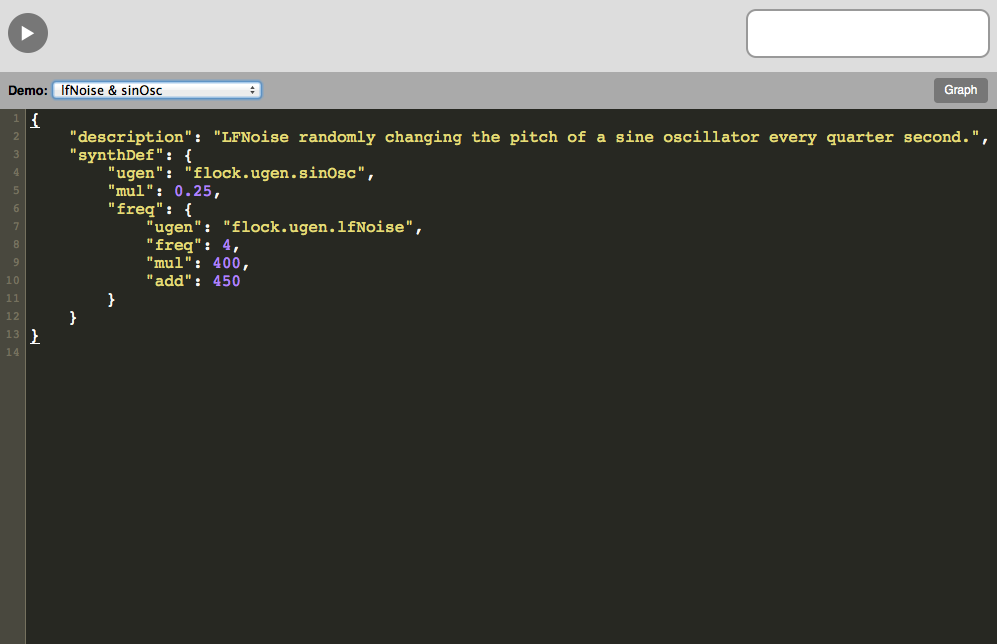
\includegraphics[width=0.9\columnwidth]{images/flocking-playground-source-view.png}
\caption{ A screenshot of Flocking's interactive programming environment.\label{fig:playground}}
\end{figure}

\begin{figure}[ht]
\centering
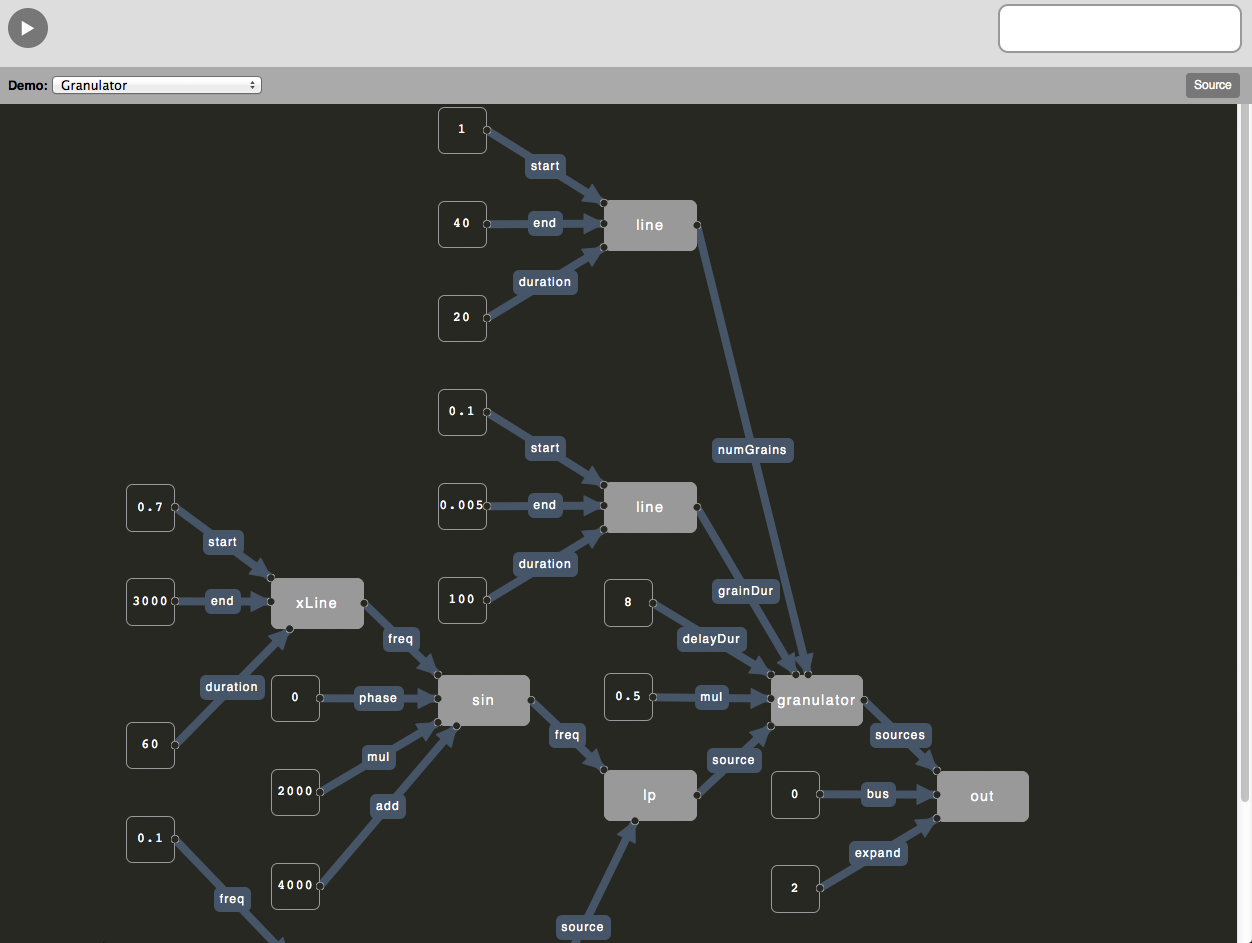
\includegraphics[width=0.9\columnwidth]{images/flocking-playground-graphical-view.png}
\caption{ A screenshot of an in-development patching GUI for Flocking.\label{fig:graphical}}
\end{figure}

The new Flocking Playground is being built with Fluid Infusion\footnote{http://fluidproject.org/products/infusion}, a JavaScript framework that supports end-user personalization and development \cite{hcii2014}. Infusion's infrastructure for relaying, transforming, and firing changes across diverse models within an application will be critical for maintaining synchronization between the graphical and source views of the Playground. We also envision that Infusion's model infrastructure will help support live coding in the Playground using an ``on the fly change merging" approach not unlike that described in Bret Victor's {\it Inventing on Principle}\cite{inventingonprinciple}. (Adam how do we cite a video in bibtex format? https://vimeo.com/36579366)

\subsection{Greater Web Audio Integration}

Due to the fact that Flocking takes control of the sample generation process directly, it uses very few features of the W3C Web Audio API. As the specification evolves, plans are underway to adopt more of its features. At the moment, Flocking consists of a single ScriptProcessorNode that is directly connected to the Web Audio API's destination sink. This currently precludes---or makes very difficult---the use of the powerful native Nodes offered by Web Audio, including the Panner, Waveshaper, and Analyser nodes.

We are in the midst of planning an updated version of the Flocking architecture that allows for Flocking unit generators to be interleaved with native Web Audio nodes. Nicknamed ``islands," this approach will make a complete separation between unit generators and synths, introducing a proxy unit generator type that adapts inputs between a native node and a Flocking unit generator.

\begin{figure}[ht]
\centering
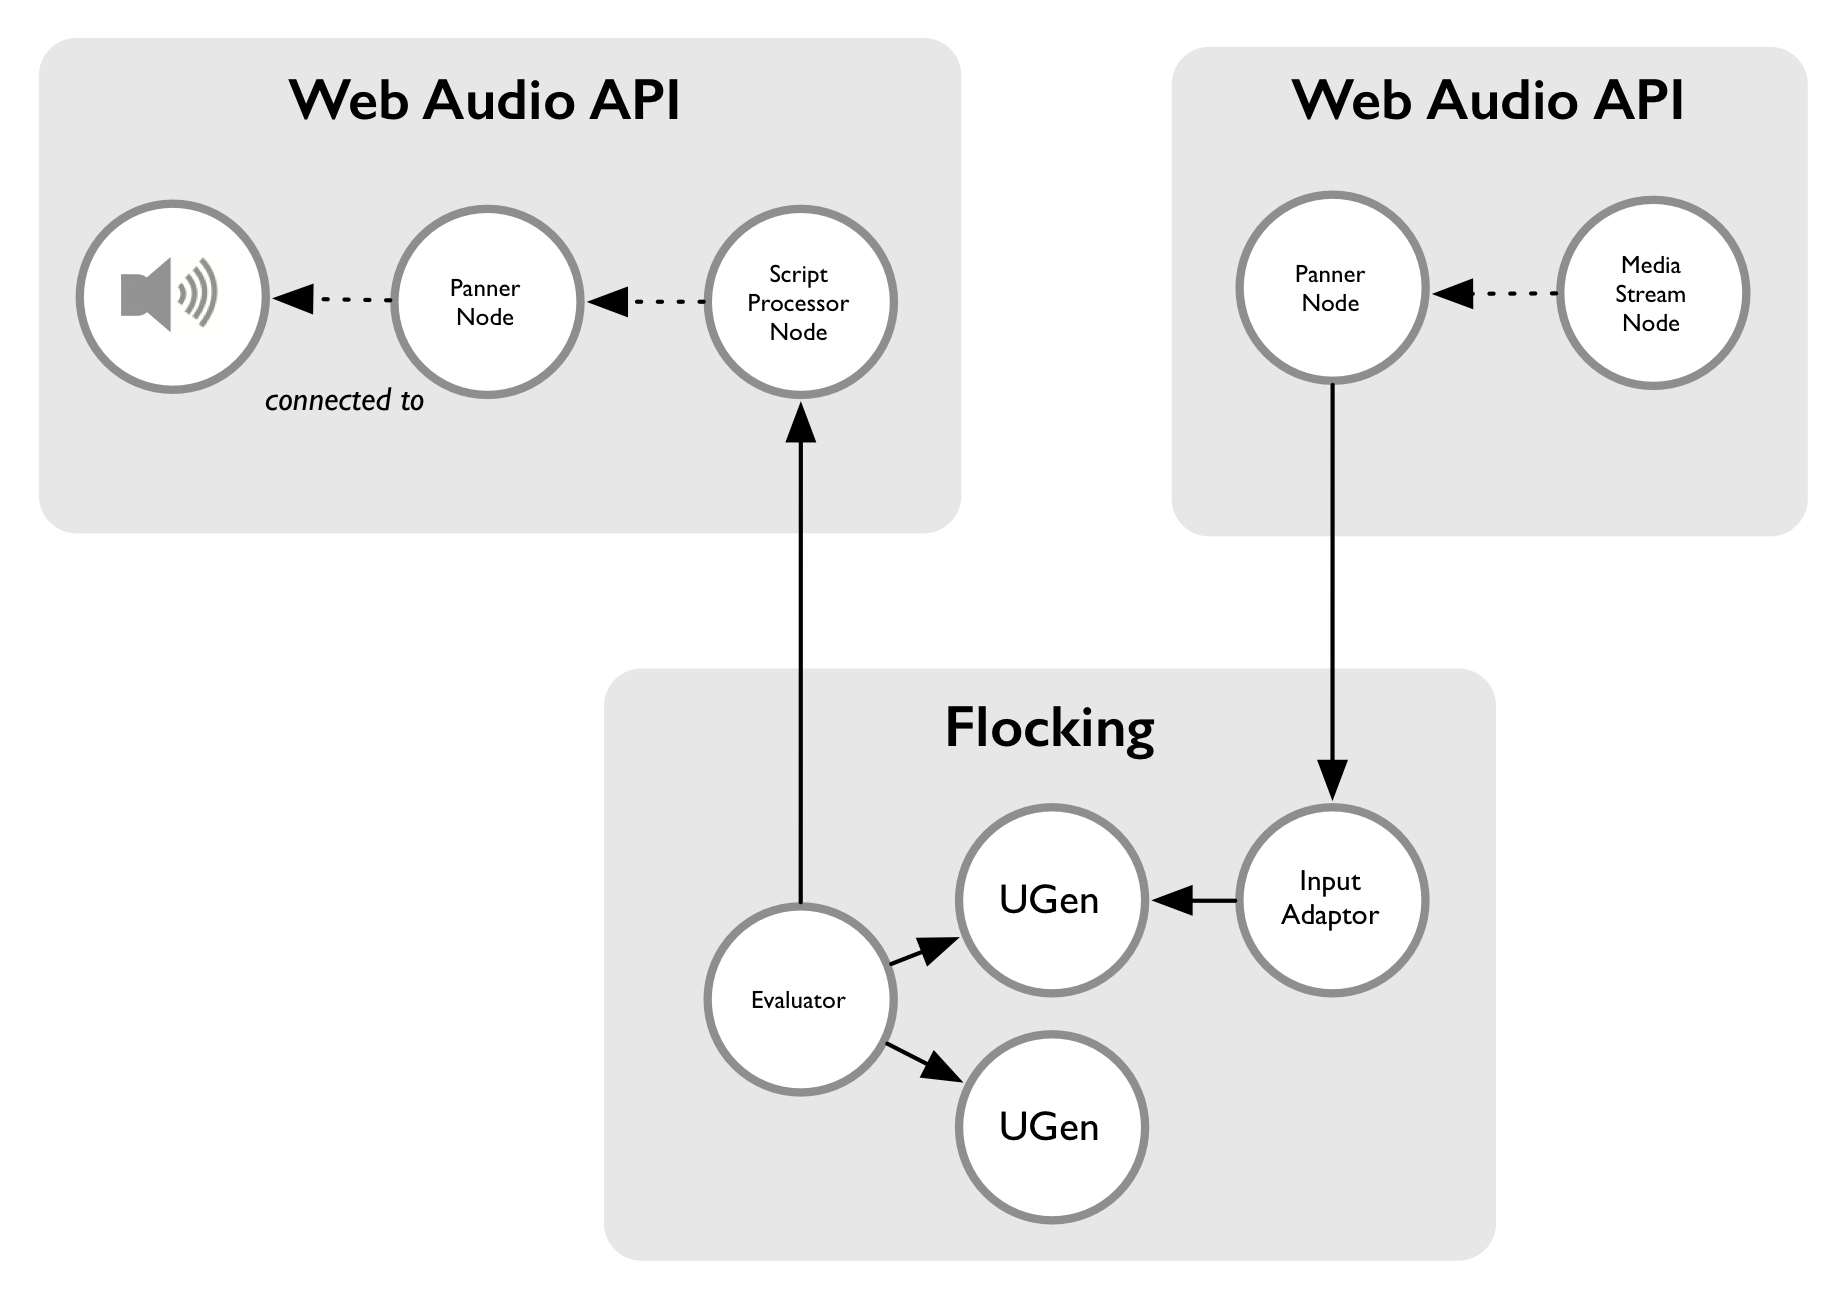
\includegraphics[width=0.9\columnwidth]{images/flocking-web-audio-islands.png}
\caption{ A diagram showing how Flocking will support mixing unit generators with native Web Audio API nodes.\label{fig:graphical}}
\end{figure}

This architecture change will also help prepare Flocking for Web Worker-based ScriptProcessorNodes, which are planned for a future version of the Web Audio specification\footnote{https://github.com/WebAudio/web-audio-api/issues/113}.

\section{Conclusions}
Awesomeness has been demonstrated.

\nocite{*} % just to put everything in reference section for now


%%%%%%%%%%%%%%%%%%%%%%%%%%%%%%%%%%%%%%%%%%%%%%%%%%%%%%%%%%%%%%%%%%%%%%%%%%%%%
%bibliography here
\bibliography{flockingbibliography}

\end{document}
